\documentclass{article}
\usepackage[margin=1in]{geometry}
\usepackage{graphicx}
\usepackage{hyperref}
\usepackage{float}
\usepackage{bookmark}
\usepackage{listings}

\title{Mini-Assignment 1: CS3423 - Compilers - II}
\author{Harsh Agarwal\\
\texttt{CS15BTECH11019}
\and S Vishwak\\
\texttt{CS15BTECH11043}}
\date{}

\begin{document}
\maketitle

\section*{Abstract}
This report is written to meet the requirements of Mini-Assignment 1 of Compilers - II. The contributions of this report are as follows: Section 1 provides a brief idea of the LLVM directory structure specifying the important files/folders in each directory. Section 2 discusses the Clang AST and its features and how to traverse the AST. Section 3 discusses the LLVM Intermediate Representation which is "the" core of the LLVM compiler architecture with some examples and an explanation of those examples as well. Section 4 discusses the LLVM Assembly Code generated in brief, Section 5 lists some well-known tools in the LLVM Compiler ToolChain, Section 6 discusses the error handling mechanism of LLVM and Section 7 provides an overview of Kaleidoscope - a toy language.

\section{LLVM Directory Structure}
\begin{flushleft}
The LLVM codebase is extremely huge and putting all the code under one shed will not be feasible or well-accessible. Hence, the LLVM Compiler Infrastructure is actually spread across a collection of multiple files and folders. These folders might consist a set of folders, which will inturn contain a set of files and folders and the it goes on and on. This is done to ensure that there is relatively less hassle while trying to find a file, and there might be multiple files with the same name, but intended for different purposes.
\(\newline\)

When you download the source code: say you are cloning it, it gets cloned into a folder named \texttt{llvm} by default. Peeking into the \texttt{llvm} directory, there are quite a few folders and almost every one of them are crucial to proper functioning of the LLVM Compiler Architecture. Below is a table that represents the important folders and the uses of them: \footnote{\href{https://llvm.org/docs/GettingStarted.html}{Getting Started with LLVM-6.0}}

\begin{center}
\begin{tabular}{|c|c|}
\hline
Path from \texttt{./llvm} & Use of the folder \\
\hline
\hline
\texttt{./docs} & Documentation for various tools present in the LLVM Compiler Infrastructure \\
\hline
\texttt{./include} & Consists of the public header files exported from the LLVM directory \\ 
\hline
\texttt{./lib} & Almost all source code for LLVM is in this directory \\
\hline
\texttt{./projects} & Used to create your own projects using LLVM \\
\hline
\texttt{./test} & Feature, regression and other sanity tests on the LLVM Compiler Infrastructure \\
\hline
\texttt{./test-suite} & Correctness, performance and benchmarking test suite for LLVM \\
\hline
\texttt{./tools} & Executables built out the source code in \texttt{./lib} \\
\hline
\texttt{./utils} & Utilities for working with LLVM source code \\
\hline
\end{tabular}
\end{center}
\(\newline\)

Let us consider the \texttt{.llvm/include/} directory. There are two main directories: \texttt{llvm} and \texttt{llvm-c}. \texttt{./llvm/include/llvm} contains all the header files and subdirectories for different parts of LLVM, whereas \texttt{./llvm/include/llvm-c} contains the code that will help provide a C API for special parts of LLVM. It may seem that \texttt{./llvm/include/llvm} may seem important, and hence on looking we seen a lot of folders again. We will be listing the subdirectories that are important according to our knowledge, and these are as follows:
\(\newline\)

\begin{center}
\begin{tabular}{|c|c|}
\hline
Path from \texttt{./llvm/include/llvm} & Use of the folder \\
\hline
\hline
\texttt{./ADT} & Headers for Abstract Data Types \\
\hline
\texttt{./Analysis} & Headers for Various Kinds of Analyses \\
\hline
\texttt{./Bitcode} & Headers for interfaces to read/write LLVM bitcodes \\
\hline
\texttt{./CodeGen} & Headers for Code Generation scheme from LLVM IRs \\
\hline
\texttt{./Configure} & Wrapper for wrapping config script \\
\hline
\texttt{./IR} & Headers for various IR related files \\
\hline
\texttt{./MC} & Headers for Machine Code support \\
\hline
\texttt{./Support} & Generic support libraries provided with LLVM \\
\hline
\texttt{./TableGen} & Table Generation Tools \\
\hline
\end{tabular}
\end{center}
\(\newline\)

Now that we have seen the headers, the corresponding main files for these headers containing the definitions can be found in \texttt{./llvm/lib}. The layout of the folders is remarkably similar to the layout of \texttt{./llvm/include/llvm}.
\(\newline\)

Now take another important directory: \texttt{./llvm/tools/}. This directory also has multitude of files and folders and \texttt{clang} is one of them. A lot of LLVM's features go into this library, and hence that is why we are looking into it. Again, we list the important directories in \texttt{./llvm/tools}.

\begin{center}
\begin{tabular}{|c|c|}
\hline
Path from \texttt{./llvm/tools} & Use of the folder \\
\hline
\hline
\texttt{./bugpoint} & To help debug optimization passes \\
\hline
\texttt{./clang} & The Clang Compiler file \\
\hline
\texttt{./llc} & LLVM Native Code Generator files \\
\hline
\texttt{./lli} & LLVM Interpreter \\
\hline
\texttt{./llvm-ar} & Archiving Utility files \\
\hline
\texttt{./llvm-as} & Low Level Assembler \\
\hline
\texttt{./llvm-bc-analyzer} & LLVM Bitcode Analyzer \\
\hline
\texttt{./llvm-c-test} & Tool for testing \texttt{llvm-c} API \\
\hline
\texttt{./llvm-dis} & Tool for disassembling LLVM assembly \\
\hline
\texttt{./link} & LLVM Linker files \\
\hline
\texttt{./opt} & Optimization options \\
\hline
\end{tabular}
\end{center}
\(\newline\)

Let's now look into some important files inside \texttt{./llvm/utils}:
\begin{itemize}
\item \texttt{codegen-diff} \(\Rightarrow\) File used to check the difference between code generated by \texttt{llc} and \texttt{lli}
\item \texttt{makellvm} \(\Rightarrow\) File used to compiles all the files in the directory and links the tool given by the first argument to \texttt{makellvm}
\item \texttt{./TableGen/} \(\Rightarrow\) Directory which tools used to generate register descriptions, instruction set descriptions and even assemblers
\end{itemize}
\end{flushleft}
\newpage


\section{The Clang Abstract Syntax Tree (Clang AST)}
\subsection{Generating the Abstract Syntax Tree}
\begin{flushleft}
The Abstract Syntax Trees are generated using the command:

\begin{center}
\texttt{clang -Xclang -ast-dump -fsyntax-only <insert\_your\_program\_name>.cpp} \footnote{\href{http://workshop.rosedu.org/2014/sesiuni/compiler/ast}{ROSEdu Workshop on Clang AST}}
\end{center}

To clarify some syntax in the above command:
\begin{itemize}
\item \texttt{-Xclang} \(\Rightarrow\) flag that the source code should be passed to the front end
\item \texttt{-fsyntax-only} \(\Rightarrow\) flag that tells Clang to stop compilation process just after building the AST
\item \texttt{-ast-dump} \(\Rightarrow\) dumps your AST
\end{itemize}

\end{flushleft}

\subsection{Structure of the AST}
\begin{flushleft}
Since the C++ grammar is huge and complicated, the Clang AST is split into 2 parts basically: The AST Part and the \texttt{ASTContext} Class. This is done to not make the Clang AST a heavy object in itself, rather storing the heavy objects elsewhere (\texttt{ASTContext} Class) and then pointing to those objects from within the AST seems like a logical option. 
\(\newline\)

The entry into the AST is via the \texttt{ASTContext} Class\footnote{Tutorial by Manuel Klimek: \href{https://www.youtube.com/watch?v=VqCkCDFLSsc}{LLVM European Meet 2013}} using the \texttt{getTranslationUnitDecl()} method.

For a given program, this can be seen when you dump the AST:
\begin{figure}[H]
\centering
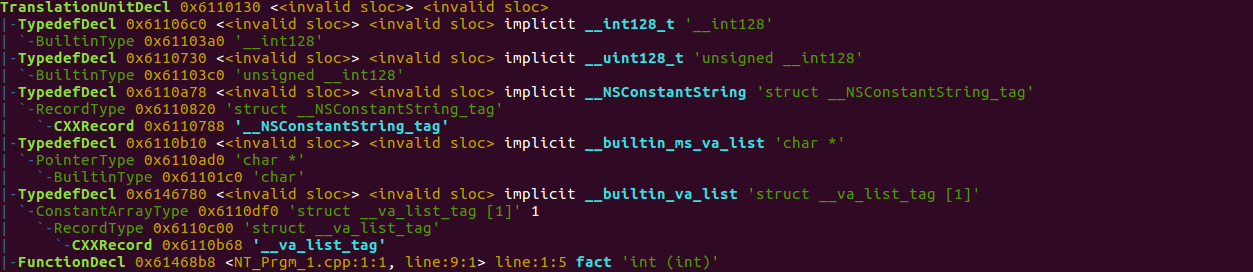
\includegraphics[width=0.6\textwidth]{./images/pic-1.png}
\end{figure}

From this starting point, you will be lead to the Core Classes of the Clang AST: \texttt{Decl} (for Declarations), \texttt{Stmt} (for Statements and Expressions), \texttt{Type} (for Types). In our programs , we do not see explicitly a AST node with a \texttt{Type} Class instance, but we see both instances of various \texttt{Decl} Classes and \texttt{Stmt} Classes. 

\subsubsection{Declarations}
So, when you encounter a Declaration, say a class, or a variable or a function, a \texttt{Decl} class instance of those items is created. Consider the below example:
\begin{figure}[H]
\centering
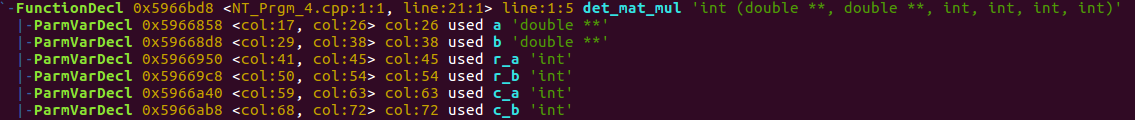
\includegraphics[width=0.6\textwidth]{./images/pic-2.png}
\end{figure}

Note how the function and the parametric variables which are a part of the function, are being declared. The name of the item (function/parametric variable) is followed by the types. For a function, you have a return type and the argument type signature of the function itself.
\begin{figure}[H]
\centering
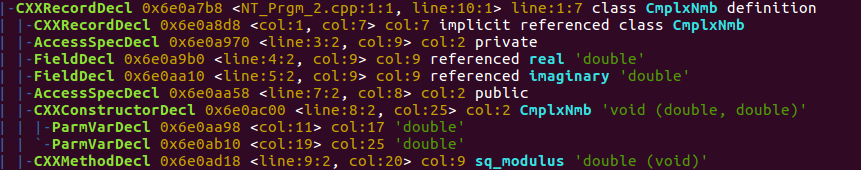
\includegraphics[width=0.6\textwidth]{./images/pic-3.png}
\end{figure}

Above is the declaration of a C++ Class. Note the declaration of Access Type Specifier and the Fields of the Class. 

\subsubsection{Statements}
Statements in the Clang AST are just as descriptive as the Declarations. There are various kinds of statements in C++, if statements, for statements, return statements. As mentioned earlier, the expressions are also contained in statements as far as Clang AST is concerned. We think that C++ has left no stone unturned in its grammar with respect to statements, and there are quite a few of them: bool expressions, cast expressions, binary expressions to name a few.
\(\newline\)

Our claim should be clear with 1-2 examples below:

\begin{figure}[H]
\centering
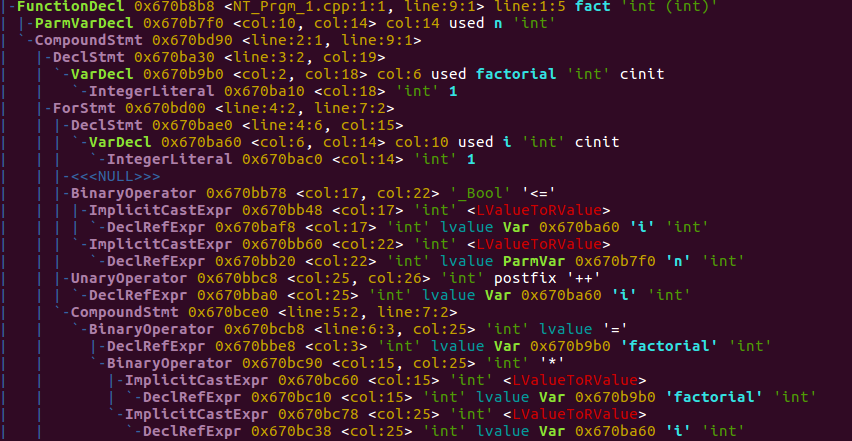
\includegraphics[width=0.6\textwidth]{./images/pic-4.png}
\end{figure}
This is a function (almost), written in C++. The violet coloured lines represent Statements. Note the different types of Statements that are being referenced here.

\begin{figure}[H]
\centering
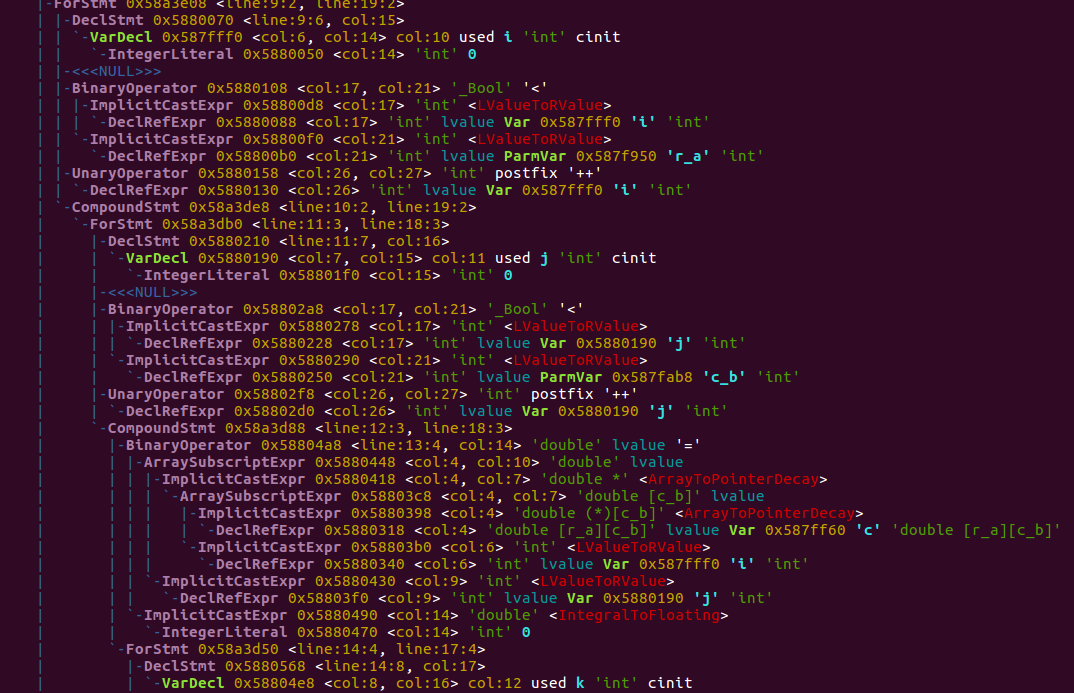
\includegraphics[width=0.6\textwidth]{./images/pic-5.png}
\end{figure}

This is a nested \texttt{for} loop (the last loop has not been shown in entirety). Notice the various Statements ranging from variable declaration in the \texttt{for} loop, and subscript expressions as well.
\(\newline\)

It is good to see how the naming in the Clang AST has been done which makes the AST more comprehensible.
\end{flushleft}

\subsection{AST Traversal}
\begin{flushleft}
We now know how complicated the C++ Grammar is, and also the intricate difficulties while trying to parse it as well. Clang does a great job by providing a size-optimized version of the AST. But how do you traverse the AST? The most common way to do it (as far as we know), is to use a AST Visitor mechanism. We take help of a AST Visitor namely, the \texttt{RecursiveASTVisitor} to help traverse the AST. As the name suggests, the \texttt{RecursiveASTVisitor} traverse the AST in a recursive manner, while covering the nodes. 
\(\newline\)

The typical \texttt{RecursiveASTVisitor} is written keeping the following information in mind: mention the nodes you want to traverse and the way you want to traverse them.
\(\newline\)

This is what makes the \texttt{RecursiveASTVisitor} so powerful \(-\) once you know how to write a \texttt{RecursiveASTVisitor}, you can dictate to pick particular types of Nodes you want to traverse to (for example: \texttt{ifStmt}, \texttt{ElseStmt} or \texttt{VarDecl}, \texttt{CxxRecordDecl}) and how you want to traverse them i.e., the order for traversal (\texttt{Stmt} instances first and the \texttt{Decl} instances or any other variant).
\(\newline\)

In more detail: the \texttt{RecursiveASTVisitor} does three tasks: \footnote{\href{https://clang.llvm.org/doxygen/RecursiveASTVisitor_8h_source.html}{Source code of \texttt{RecursiveASTVisitor.h}}}
\begin{enumerate}
\item Traverses the AST
\item At a given node, walk up to the class hierarchy (from the node’s dynamic type) to one of the “core” classes : \texttt{Decl}, \texttt{Stmt}, \texttt{Type}, depending on the code.
\item Call a user function to actually visit the node.
\end{enumerate}

How are these tasks done? These tasks are accomplished using the following methods:
\begin{itemize}
\item \texttt{Traverse<insert\_core\_class>} for task 1.
\item \texttt{WalkUpFrom<insert\_name\_of\_class>} for task 2
\item \texttt{Visit<insert\_name\_of\_class>} for task 3
\end{itemize}

There also exists a hierarchy in these methods. \texttt{Traverse >> WalkUpFrom >> Visit}. \texttt{Traverse} is the highest in this hierarchy, meaning it can call a \texttt{WalkUpFrom} method or \texttt{Visit} method, whereas \texttt{Visit} is the lowermost in the hierarchy and it cannot call any higher methods.
\(\newline\)

This \texttt{RecursiveASTVisitor} also tries to visit every node of the source code exactly once, which also makes it powerful. The \texttt{RecursiveASTVisitor} uses a visitor design principle in its implementation. This enables modularity in the code and helps add new features/methods in the existing code, without altering the base code/classes.
\end{flushleft}

\newpage
\section{The LLVM Intermediate Representation (IR)}
\subsection{Introduction}
\begin{flushleft}
LLVM is a Static Single Assignment (SSA) based representation that provides type safety, low-level operations, flexibility, and the capability of representing all high-level languages in a clean manner. LLVM has many other way to represent a program (making them a IR as well), but the LLVM IR is the IR defined by the \texttt{Instruction} class (the base class for all of the LLVM instructions). 
\(\newline\)

Although it is known that the LLVM IR is (mostly) target independent, there are certain parts of LLVM which is target dependent. The reasons of the existence such parts are:
\begin{itemize}
\item The LLVM IR uses some special library calls, sizes of the various data types, calling conventions which are attributes defined by the target architecture.
\item Some C header files contain some hardware dependent macros/functions which match the kernel syscalls, thereby making LLVM IR a bit target dependent.
\end{itemize}
\end{flushleft}

\subsection{Generating the LLVM IR}
\begin{flushleft}
The LLVM IR is generated using the command:
\begin{center}
\texttt{clang -S -emit-llvm <insert\_your\_program\_name>.cpp}\footnote{\href{https://clang.llvm.org/get_started.html}{Getting Started with Clang}}
\end{center}

This command generates a file with the same name as the entered program, but the file extension is \texttt{.ll}.

\end{flushleft}
\subsection{Some special LLVM IR Features}
\subsubsection{Attributes}
\begin{flushleft}
Each function in the LLVM IR has a set of attributes explaining its characteristics and some target specific information. The attributes variable start with \texttt{\#}.
\(\newline\)

Below is a list of some attributes and a brief explanation of them:
\begin{itemize}
\item \texttt{optnone} \(\Rightarrow\) This tells whether compilation was done using optimizations flags or not
\item \texttt{nounwind} \(\Rightarrow\) This indicates that the function never raises an exception
\item \texttt{norecurse} \(\Rightarrow\) This function attribute indicates that the function does not call itself either directly or indirectly down any possible call path
\item \texttt{noinline} \(\Rightarrow\) This attribute indicates that the inliner should never inline this function in any situation
\item \texttt{argmemonly} \(\Rightarrow\) This attribute indicates that the only memory accesses inside function are loads and stores from objects pointed to by its pointer-typed arguments, with arbitrary offsets
\item \texttt{noalias} \(\Rightarrow\) This indicates that objects accessed via pointer values based on the argument or return value are not also accessed, during the execution of the function, via pointer values and not based on the argument or return value
\end{itemize}
\end{flushleft}

\subsubsection{Functions}
\begin{flushleft}
Every function starts with entry basic block and this entry basic block should not be the target of any branch instruction and every basic block has a terminator instruction, one that jumps to other basic blocks or returns from the function (return from a function using the \texttt{ret} command). 
\end{flushleft}

\subsubsection{Some miscellaneous points worth noting}
\begin{flushleft}
If we compile a program without any optimizations and a function in that program has arguments (say n), the procedure followed is:
\begin{enumerate}
\item First n pointers are allocated to the function stack frame.
\item The value of arguments are stored in the stack at the allocated locations.
\item The n values stored in the stack are loaded into local variables.
\item The remaining function body steps follow.
\end{enumerate}

If the same program is compiled with optimizations, then the actual parameters are directly used (after specifying \texttt{local\_unnamed\_addr} in the function definition).
\(\newline\)

Another key observation was that the \texttt{signed} and \texttt{unsigned} characteristics is not taken into account when allocating memory. This observation comes from the line of code:
\begin{center}
\texttt{global i32 -10, align 4}
\end{center}
which occurs regardless of whether the variable is \texttt{signed} or \texttt{unsigned}. In fact, this characteristic is actually taken care of in the operators operate that over these variables. LLVM IR has specific arithmetic functions for both \texttt{signed} and \texttt{unsigned} variables.
\(\newline\)
\end{flushleft}

\subsection{Understanding LLVM IR for some programs}
\subsubsection{Program 1}
\begin{flushleft}
This program uses a recursive function to calculate the \(n^{th}\) Fibonacci number\footnote{\ref{p1}}. We takeaway a few points:
\begin{itemize}
\item The function name is changed \texttt{\_Z3fibi} , where \texttt{fib} is the function name. \texttt{\_Z3} is a label added by LLVM IR and \texttt{i} (following the function name) denotes the existence of 1 integer type argument. In the case of the same function written in C, the function name remains \texttt{fib} (as there is no function overloading in C).
\item The function attributes of \texttt{fib} function are \texttt{noinline}, \texttt{optnone}, \texttt{uwtable}. \texttt{norecurse} attribute is not there as this function involves recursion.
\item For recursive functions and main function (tested for factorial program also) first command in the entry basic block is always \texttt{\%retval = alloca i32, align 4}, denoting the memory for the return value is allocated first.
\item When compiling with \texttt{-O3} flag, the recursive call becomes tail call.
\end{itemize}
\end{flushleft}

\subsubsection{Program 2}
\begin{flushleft}
This program uses a iterative function to calculate the \(n^{th}\) Fibonacci number\footnote{\ref{p2}}. Points to be noted are:
\begin{itemize}
\item The function attributes of \texttt{fib} function are \texttt{noinline}, \texttt{nounwind}, \texttt{optnone} and \texttt{uwtable}.
\item Each loop has 4 Basic Blocks namely, \texttt{loop.cond}, \texttt{loop.body}, \texttt{loop.inc} and \texttt{loop.end}.
\item \texttt{label} is a primitive datatype in LLVM IR, and branching is done as \texttt{br label \%for.cond}.
\end{itemize}
\end{flushleft}

\subsubsection{Program 3}
\begin{flushleft}
This program calculates the sum of an array\footnote{\ref{p3}}. We takeaway a few points:
\begin{itemize}
\item Array datatype is declared as \texttt{[\#elements \(\times\) type\_of\_element]}.
\item \texttt{\_ZZ4mainE1a} attributes are \texttt{noinline}, \texttt{norecurse}, \texttt{nounwind}, \texttt{optnone} and \texttt{uwtable}.
\item If there is a constant array i.e., \texttt{int a[] = \{1,2,3,4,5\}}, \texttt{@\_ZZ4mainE1a = private unnamed\_addr constant [6 \(\times\) i32] [i32 1, i32 4, i32 6, i32 -5, i32 0, i32 12], align 16} is declared outside any function.
\item For copying \texttt{@\_ZZ4mainE1a} into the main function, \texttt{\%0 = bitcast [6 \(\times\) i32]* \%a to i8*} is done, which changes array pointer \texttt{\%a} to \texttt{i8} pointer without changing the bits.
\item Array element is accessed as follows: first \texttt{\%idxprom = set i32 \%2 to i64} takes place, which changes \texttt{\%2} from \texttt{i32} to \texttt{i64}. Then element is accessed via \texttt{getelementptr} \texttt{inbounds}.
\end{itemize}
\end{flushleft}

\subsubsection{Program 4}
\begin{flushleft}
This program experiments with Structures, Unions and Enumerations\footnote{\ref{p4}}. Some observations were:
\begin{itemize}
\item A struct type is allocated as \texttt{type {type1,type2,...}} and the variable name starts with \texttt{struct}. Example: \texttt{\%struct.node = type {i32, \%struct.node*}}.
\item There are 2 types of structures in LLVM IR, normal struct type and packed struct type.
\item The enumerator type in C is translated to its values and in LLVM IR its occurrence is replaced by its mapped number. There is no specific type for enumerator in LLVM IR.
\item For Union type, a structure is allocated of type of that field in union that has maximum size.
\item \texttt{getelementptr} function is used to calculate the memory address where the value is stored.
\end{itemize}
\end{flushleft}

\subsubsection{Program 5}
\begin{flushleft}
This program discusses string manipulation\footnote{\ref{p5}}. Some observations were:
\begin{itemize}
\item Functions from header files are just declared. They are not defined in the IR. There definitions are present in the header files.
\item \texttt{strlen} has attributes \texttt{nounwind} and \texttt{readonly}.
\item \texttt{char} type is actually \texttt{i8} in LLVM IR.
\item \texttt{strlen} returns \texttt{i64} type and this is truncated to \texttt{i32} type.
\end{itemize}
\end{flushleft}

\newpage
\section{The LLVM Assembly Code}
\subsection{Introduction}
\begin{flushleft}
In compiler construction, name mangling\footnote{\href{https://en.wikipedia.org/wiki/Name\_mangling}{Wikipedia definition}} is a technique used to solve various problems caused by the need to resolve unique names for programming entities in many modern programming languages.
\(\newline\)

In the case of C++, Since function overloading is allowed in C++ the function names are converted to a representation similar to LLVM IR C++ function representation. The Assembly function name consists of 3 parts:
\begin{itemize}
\item \texttt{\_Zn}, where \texttt{n} is a natural number.
\item Function Name \(\Rightarrow\) This is the same name as given in the C++ name.
\item Parameters :\(\Rightarrow\) Every data type has a specific representation on assembly. After the function name every argument representation is appended.
\end{itemize}

For example: \texttt{int add(int a, int b)} is translated to \texttt{\_Z3addii}. Below is table of representations of datatypes in the Assembly language:

\begin{center}
\begin{tabular}{|c|c|}
\hline
C++ Datatype & Assembly Representation \\
\hline
\hline
\texttt{int} & \texttt{i} \\
\hline
\texttt{float} & \texttt{f} \\
\hline
\texttt{double} & \texttt{d} \\
\hline
\texttt{char} & \texttt{c} \\
\hline
\texttt{int*} & \texttt{Pi} \\
\hline
\texttt{float*} & \texttt{Pf} \\
\hline
\texttt{double*} & \texttt{Pd} \\
\hline
\texttt{char*} & \texttt{Pc} \\
\hline
\end{tabular}
\end{center}
Name mangling is not done in C, since function overloading is not supported.
\end{flushleft}

\subsection{Certain \texttt{x86\_64} Assembly Characteristics}
\begin{flushleft}
Every \texttt{.s} files begins with a \texttt{.text} section and a \texttt{.file} section where it tells about the information of the C file from which the assembly code was generated. At the beginning of every function there is a \texttt{.globl} section which contains the function name (following the name mangling criterion state above), \texttt{.type} section of the form \texttt{func\_name@function} stating the type of the following lines and some alignment information.
\(\newline\)

There are some default CFI directives in the assembly file which store some additional information about the program, for debugging purposes. These directives can be disabled by compiling \texttt{-fno-asynchronous-unwind-tables} flag during compilation. These directives can be used to trace back the function calls across all the functions. Some common CFI directives are mentioned below:
\begin{itemize}
\item \texttt{cfi\_startproc} \(\Rightarrow\) This is used at the beginning of each function that should have an entry in \texttt{.eh\_frame}. It initializes some internal data structures. This information is used for exception handling and making debug calling stack faster.
\item \texttt{cfi\_endproc} \(\Rightarrow\) This denotes the end of \texttt{cfi\_startproc} block.
\item \texttt{cfi\_def\_cfa\_offset} \(\Rightarrow\) This modifies a rule for computing CFA. Register remains the same, but offset is new.
\item \texttt{cfi\_def\_cfa\_register} \(\Rightarrow\) This modifies a rule for computing CFA by changing the register that will be used instead of the old one.
\end{itemize}

There are many registers in the \texttt{x86\_64} architecture\footnote{\href{http://www.hep.wisc.edu/~pinghc/x86AssmTutorial.htm}{\texttt{x86} tutorial}}. Some important processor ones are listed below:
\begin{itemize}
\item \texttt{EAX}, \texttt{EBX}, \texttt{ECX}, \texttt{EAX} \(\Rightarrow\) intended for general purpose, more or less interchangeable.
\item \texttt{EBP} \(\Rightarrow\) used to access data on stack.
\item \texttt{ESI}, \texttt{EDI} \(\Rightarrow\) index registers, relative to \texttt{DS}, \texttt{ES} respectively.
\item \texttt{SS}, \texttt{DS}, \texttt{CS}, \texttt{ES}, \texttt{FS}, \texttt{GS} \(\Rightarrow\) segment registers of size 16 bits.
\item \texttt{EIP} \(\Rightarrow\) Program Counter (instruction pointer), relative to \texttt{CS}.
\item \texttt{ESP}, \texttt{RSP} \(\Rightarrow\) stack pointer, relative to \texttt{SS}.
\item \texttt{EFLAGS} \(\Rightarrow\) condition codes, a.k.a. Flags.
\end{itemize}

All register names used as operands must be preceded by a percent (\texttt{\%}) sign, and instruction names usually end in either \texttt{l}, \texttt{w}, or \texttt{b}, indicating the size of the operands: \texttt{long} (32 bits), \texttt{word} (16 bits), or \texttt{byte} (8 bits), respectively. All the function local variables are allocated some memory in the function stack frame at the beginning of each function. Hence variable names are not stored in assembly. Certain functions to move data across registers are there like \texttt{movl} (move contents of source register to destination register), \texttt{pushl} (push \texttt{long} to stack), \texttt{popl} (pop \texttt{long} from stack), etc. Certain arithmetic functions are also provided like \texttt{addl} (add contents of source and destination register and save in destination register), \texttt{subl}, \texttt{mull}, etc.
\end{flushleft}
\newpage

\section{Playing with the Compiler Toolchain and Options}
\begin{flushleft}
There are plenty of options in LLVM to play around with. We used a few of them:
\begin{itemize}
\item \texttt{llvm-as} \(\Rightarrow\) This command converts LLVM human readable IR (\texttt{.ll}) to bitcode (\texttt{.bc}). 
\item \texttt{llvm-dis} \(\Rightarrow\) This command is the opposite of \texttt{llvm-as} i.e., 	it converts LLVM bitcode (\texttt{.bc}) to human-readable intermediate representation (\texttt{.ll}).
\item \texttt{llvm-extract} \(\Rightarrow\) This command takes a function name and extracts it from the specified LLVM bitcode file.
\item \texttt{llc} \(\Rightarrow\) This command compiles LLVM source inputs into assembly language for a specified architecture.
\item \texttt{lli} \(\Rightarrow\) This command directly executes programs in LLVM bitcode format using a just-in-time compiler or an interpreter.
\item \texttt{llvm-stress} \(\Rightarrow\) The \texttt{llvm-stress} tool is used to generate random \texttt{.ll} files.
\end{itemize}
\end{flushleft}

\subsection{Some outputs}
\begin{figure}[H]
\centering
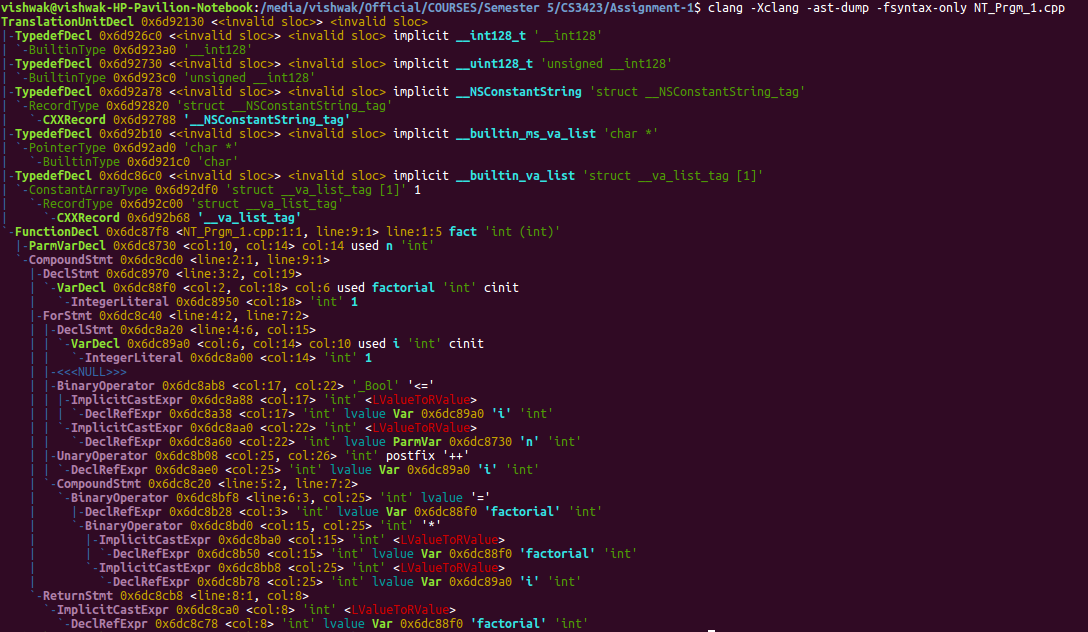
\includegraphics[width=0.7\textwidth]{./images/NT_1_AST.png}
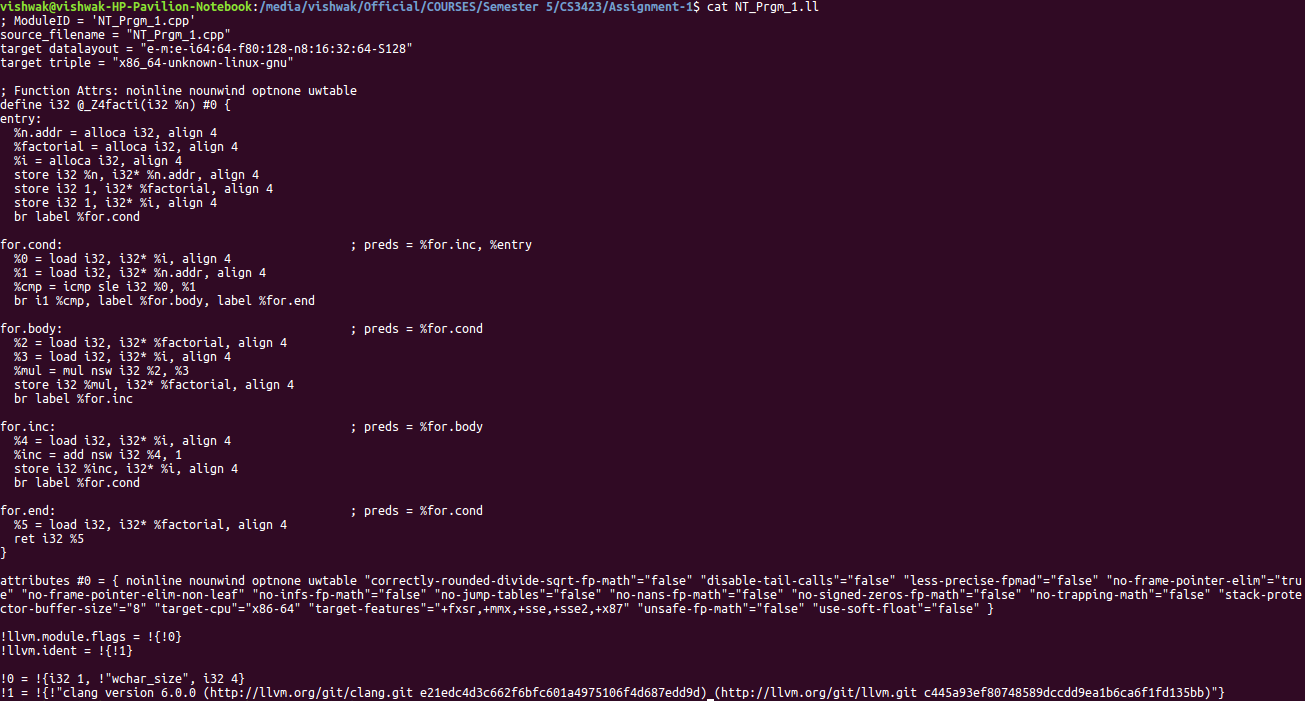
\includegraphics[width=0.7\textwidth]{./images/NT_1_IR.png}
\caption{Top to Bottom: AST, Intermediate Representation for program \ref{p6}}
\end{figure}

\begin{figure}[H]
\centering
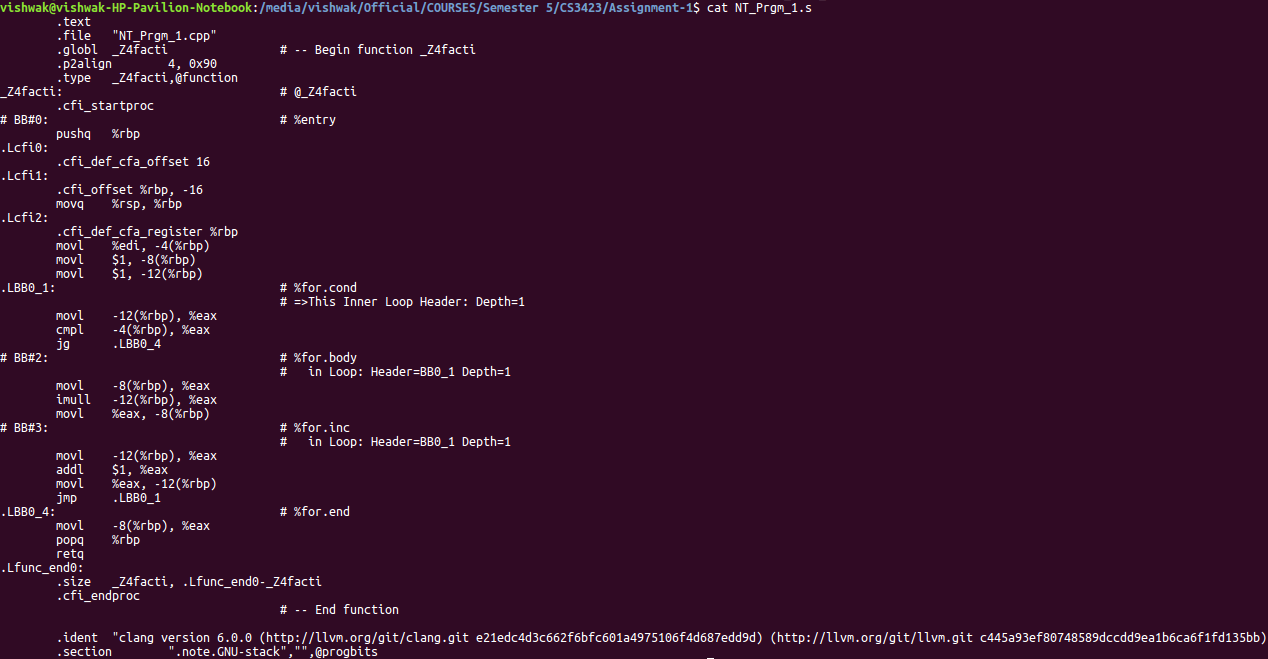
\includegraphics[width=0.7\textwidth]{./images/NT_1_ASM.png}
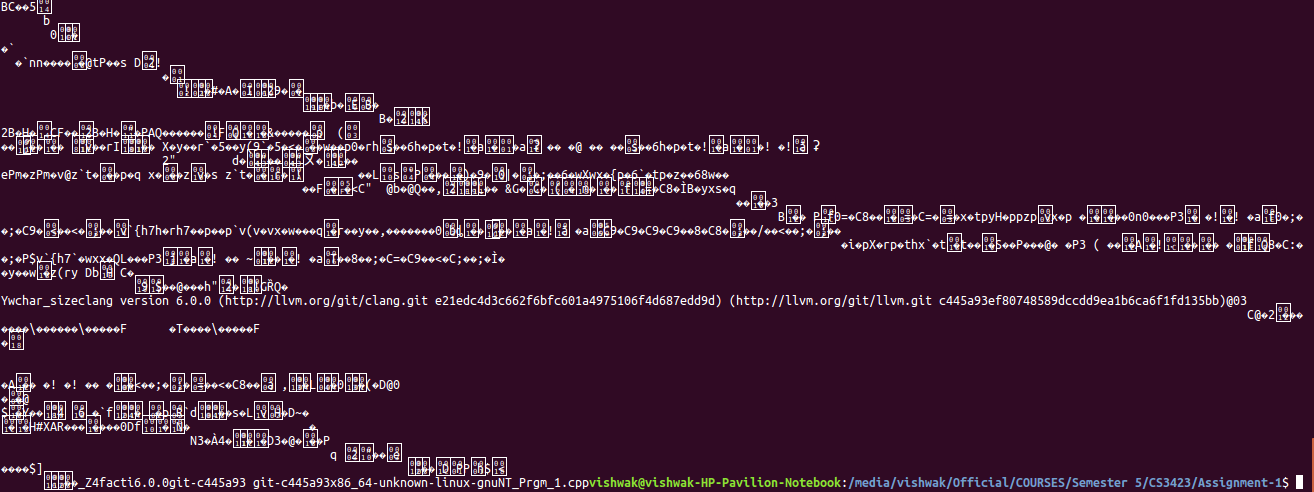
\includegraphics[width=0.7\textwidth]{./images/NT_1_BC.png}
\caption{Top to Bottom: Assembly code, Bitcode for program \ref{p6}}
\end{figure}

\section{Error Messages in LLVM}
\begin{flushleft}
Error handling is an essential part of any project. Errors fall into two broad categories: \textit{programmatic} and \textit{recoverable}. LLVM handles programmatic errors by using \texttt{assert()} and \texttt{llvm\_unreachable()}. 

Some error messages that we noticed were:
\begin{itemize}
\item \texttt{getOperand() out of range!} \(\Rightarrow\) Found at \texttt{include/llvm/CodeGen/MachineInstr.h (Line\# 285, 289)} and \texttt{include/llvm/CodeGen/User.h (Line\# 155)}.
\item \texttt{Invalid exception number} \(\Rightarrow\) Found at \texttt{/tools/clang/include/clang/AST/Type.h (Line\# 3403)}.
\item \texttt{Cannot retrieve a NULL type pointer} \(\Rightarrow\) Found at \texttt{/tools/clang/include/clang/AST/Type.h (Line\# 630)}.
\item \texttt{removing from empty list} \(\Rightarrow\) Found at \texttt{/tools/clang/include/clang/AST/DeclContextInternals.h (Line\# 106)}.
\end{itemize}

Assertions are used to express invariant conditions, and should include a message describing the invariant. The syntax for \texttt{assert()} is \texttt{assert(condition \&\& ERROR\_MESSAGE)}. But in the release mode assertions are disabled by default. \texttt{llvm\_unreachable()} can be used document areas of control flow that should never be entered if the program invariants hold.
\end{flushleft}

\section{Kaleidoscope - A Brief Case Study}
\begin{flushleft}
Kaleidoscope is a toy language defined to illustrate how LLVM can be used to implement other languages. Kaleidoscope is a procedural programming language with only 1 datatype: 64-bit floating point number. This makes Kaleidoscope a language with syntax simplicity.

\subsubsection{Lexer}
Since the language is extremely minimalistic, the number of actual 'keywords' are few (5 in number). If encounter any other token other than keywords, then a unique numerical value is returned, typically the ASCII value. There are five tokens: \texttt{tok\_eof}, \texttt{tok\_def}, \texttt{tok\_extern}, \texttt{tok\_identifier} and \texttt{tok\_number}. The content of the tokens \texttt{tok\_identifier} and \texttt{tok\_number} are a \texttt{string} and \texttt{double} value in C++ respectively.
\(\newline\)

A lexer is implemented easily with a single loop. We read the space separated words in the code as a token. We then compare the tokens for any keywords, and return the values pertaining to them if detected.

\subsubsection{Parser}

Again, due to the extremely minimalistic nature of Kaleidoscope, there are only 3 different constructs in the language: expressions, prototype and function object. We then define a separate class for each construct, just like how it is done in Clang. Then each construct has a set of sub-constructs which are defined by inheriting the properties of the parent class.
\(\newline\)

After obtaining the class definitions for the constructs and the children sub-constructs, we proceed to build a AST. We make use of the LLVM node creation routine \texttt{make\_unique} to create the nodes. In the case of binary operations we give the binary operator and the precedence as a pair \texttt{(char, int)} to the parser so that the precedence is taken care of. At the end, we use a simple recursive main loop to parse the file.

\subsubsection{Intermediate Representation}
Once the parser is done, we generate the LLVM IR. This is not as easy as the Lexer or the Parser, but could have been more complicated if not for the LLVM infrastructure. The LLVM compiler infrastructure provides us with a nice \texttt{IRBuilder} class, wherein you can add different types of instructions. \texttt{TheModule} is another construct provided by LLVM to help contains the functions and global variables.
\(\newline\)

This API provides a platform to create and inserting instructions into a \texttt{BasicBlock}: either at the end of a \texttt{BasicBlock} or within a specific location in a block. A \texttt{BasicBlock} is essentially a set of instructions that execute sequentially one after the other.
\(\newline\)

\(\newline\)

From the set of examples that was given in the LLVM IR, it is valid to ask if this the IR generated by LLVM for Kaleidoscope work the same way on different targets i.e., architectures? The answer is yes, and this is one key property of LLVM known as target independence\footnote{\href{https://llvm.org/docs/tutorial/LangImpl10.html}{Target Independence in LLVM IR}}. This means that, if we write Kaleidoscope code on a ARM machine and compile this IR on a x86 machine, then there will be no problems at all. This is because the LLVM IR is target independent, which helps performs machine independent optimizations in an easier fashion. We discussed about LLVM's target dependency, and for a minimalistic language like Kaleidoscope, we think that there shouldn't be problems at all.
\(\newline\)

Also from the source code used to demonstrate the Kaleidoscope IR generation, it can be seen that LLVM arbitrarily allows unsafe pointer casts. Although we have not discussed about Garbage Collectors (GCs), the LLVM compiler infrastructure has support for GCs as well.
\end{flushleft}

\newpage
\section*{Appendix}
This section has the source codes for the examples explained with in Section 3.4 and 5.1.

\subsection{Program for Section 3.4.1}
\begin{flushleft}
\label{p1}
\begin{lstlisting}
int fib(int n) {
	if(n<=1)
		return 1;
	return fib(n-1)+fib(n-2);
}

int main() {
	int a;
	a = fib(5);
}
\end{lstlisting}
\end{flushleft}

\subsection{Program for Section 3.4.2}
\begin{flushleft}
\label{p2}
\begin{lstlisting}
int fib(int n) {
	int a = 1, b = 1, c;
	for(int i = 2;i <= n; i++) {
		c = a+b;
		a=b;
		b=c;
	} 
	return c;
}

int main() {
	int a = fib(5);
}
\end{lstlisting}
\end{flushleft}

\subsection{Program for Section 3.4.3}
\begin{flushleft}
\label{p3}
\begin{lstlisting}
int main() {    
    int a[] = {1,2,3,4,5,6};
	int sum = 0;
	for(int i=0;i <6; i++) 
		sum += a[i];
    return 0;
}
\end{lstlisting}
\end{flushleft}
\newpage

\subsection{Program for Section 3.4.4}
\begin{flushleft}
\label{p4}
\begin{lstlisting}
#include <stdio.h>

struct node
{
	int val;
	struct node* next;
};

enum week{Mon, Tue, Wed};

union temp {
	int a;
	int b;
	struct node c;
};

int main() {
	struct node obj;
	obj.val = 4;
	obj.next = NULL;

    enum week day;
    day = Wed;
 	day = Mon;

 	union temp obj2;
       
}
\end{lstlisting}
\end{flushleft}

\subsection{Program for Section 3.4.5}
\begin{flushleft}
\label{p5}
\begin{lstlisting}
#include <stdio.h>
#include <string.h>

int main()
{
	char a[] = "This is LLVM IR";
	for (int i = strlen(a); i >= 0 ; --i)
	{
		printf("%c", a[i]);
	}
	return 0;
}
\end{lstlisting}
\end{flushleft}
\newpage

\subsection{Program for Section 5.1}
\begin{flushleft}
\label{p6}
\begin{lstlisting}
int fact(int n)
{
	int factorial = 1;
	for(int i = 1; i <= n; i++)
	{
		factorial	= factorial*i;
	}
return factorial;
}
\end{lstlisting}
\end{flushleft}
\end{document}
